\documentclass{article}

\usepackage{cite}
\usepackage{amsmath}
\usepackage[pdftex]{color,graphicx}
\usepackage{verbatim}
\usepackage{hyperref}

\setlength\topmargin{-0.5in}
\setlength\headsep{0in}
\setlength\textwidth{6.5in}
\setlength\textheight{9in}
\setlength\oddsidemargin{0in}
\setlength\evensidemargin{0in}

\title{NETPLAN V2.0.1 User Manual}
\author{Eduardo Ibanez}


\begin{document}

\maketitle
\tableofcontents


\section{Introduction}

This document serves as an introduction to the use of NETPLAN, including how to download, access and execute the software. It is intended to cover the basic ideas from a user point of view. For more information you may visit the NETPLAN website\footnote{\url{http://github.com/eibanez/NETPLAN}}.

Whenever possible, the connection between then model and the implementation for variables and parameters is included. As always, I appreciate your feedback and help to correct mistakes or to make the document easier to understand.


\section{Setting up}

Please download the code corresponding to latest version of NETPLAN from the \href{http://github.com/eibanez/NETPLAN}{NETPLAN website}. Extract its content to a folder called \verb=netplan= in your ISU ``My documents". We will use these files throughout this document.

You may download one of the example ``data'' folders or create your own with the help of this manual instructions.


\subsection{Accesing Cplex}

CPLEX resides on several ISU servers, which are listed in the following URL, under the Linux categories: \url{http://it.eng.iastate.edu/remote}. To access any of them, you will need a telnet facility. I suggest using PuTTY, which is a free implementation of Telnet and SSH for Win32 and Unix platforms, along with an xterm terminal emulator.\footnote{This section has been adapted from Dr. James McCalley's class notes}

The following steps are necessary to connect to those servers:
\begin{enumerate}
  \item Download PuTTY from \url{http://clue.eng.iastate.edu/downloads.shtml}. Alternatively, the official PuTTY page is \url{http://www.chiark.greenend.org.uk/~sgtatham/putty/}. At this page, you will find some alternatives; I used (successfully) the installer, \verb=putty-0.60-installer.exe=.

  \item Run PuTTY and get the window shown in Fig.~\ref{fig:putty}. Input the name of the server in the Host Name, e.g., \verb=linux-8.ece.iastate.edu=.
\begin{figure}[ht]
\begin{center}
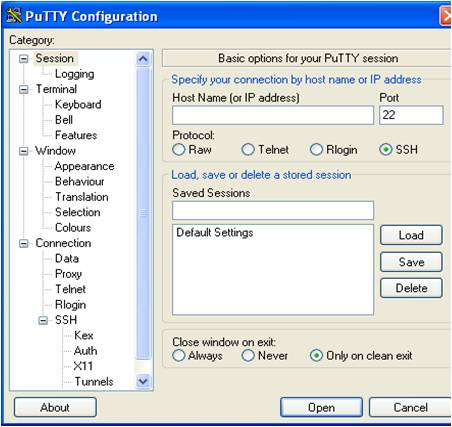
\includegraphics{figs/putty}
\end{center}
\caption{Running PuTTy}
\label{fig:putty}
\end{figure}

  \item Use your ISU username and password to log in. You will find yourself on a UNIX terminal emulator.
\end{enumerate}


\subsection{Setting the default folder}

Once you are logged in the server, use the following commands to access your \verb=netplan= folder that you previously created:
\begin{verbatim}
cd YOUR_USERNAME
cd My\ Documents
cd netplan
\end{verbatim}


\subsection{NETPLAN folder}

When you open the \verb=netplan= folder you will find these folders and files:
\begin{itemize}
  \item \verb=data=: Folder that stores the model that is being tested
  \item \verb=data/events=: Folder with the definition of events for resiliency analysis
  \item \verb=manual=: This manual and the files used to produce it
  \item \verb=src=: Folder with NETPLAN source code
  \item \verb=src/nsga2=: Folder with NSGA-II implementation on a single machine
  \item \verb=src/nsga2b=: Folder with parallelization code for NSGA-II (under development)
  \item \verb=CHANGELOG=: Text file to keep track of latest changes
  \item \verb=Makefile=: File used to simplify the compilation procedure
\end{itemize}

During the execution, two more folders called \verb=prepdata= and \verb=nsgadata= will be created. The first one is used to store auxiliary files used during the optimization and most of the results. The latter will contain the results from the NSGA-II multiobjective obtimizations.

The source code in the \verb=src= folder is divided into different modules. The main files (programs that you run) are the following:

\begin{itemize}
  \item \verb=preprocessor.cpp=: Takes information from \verb=data= folder  and creates MPS and temporary files
  \item \verb=postprocessor.cpp=: Takes MPS files and solves problem, writes solution in files
\end{itemize}

The source code in the \verb=src= folder is divided into different stages, as presented in Fig.~\ref{fig:software_implement}. The main files (programs that you run) are the following:

\begin{itemize}
  \item \verb=preprocessor.cpp= (stage 1):Takes information from \verb=data= folder  and creates MPS and temporary files
  \item \verb=postprocessor.cpp=: Takes MPS files and solves problem, writes solution in files (for checking purposes)
  \item \verb=nsga2/main.cpp= (stage 2): Main file for the NSGA-II implementation, which takes the MPS and auxiliary files and solve the multiobjective problem
  \item \verb=postnsga.cpp= (stage 3): Reads the individuals that form the Pareto front of solution and reports the solutions.
\end{itemize}

\begin{figure}[htp] \centering
  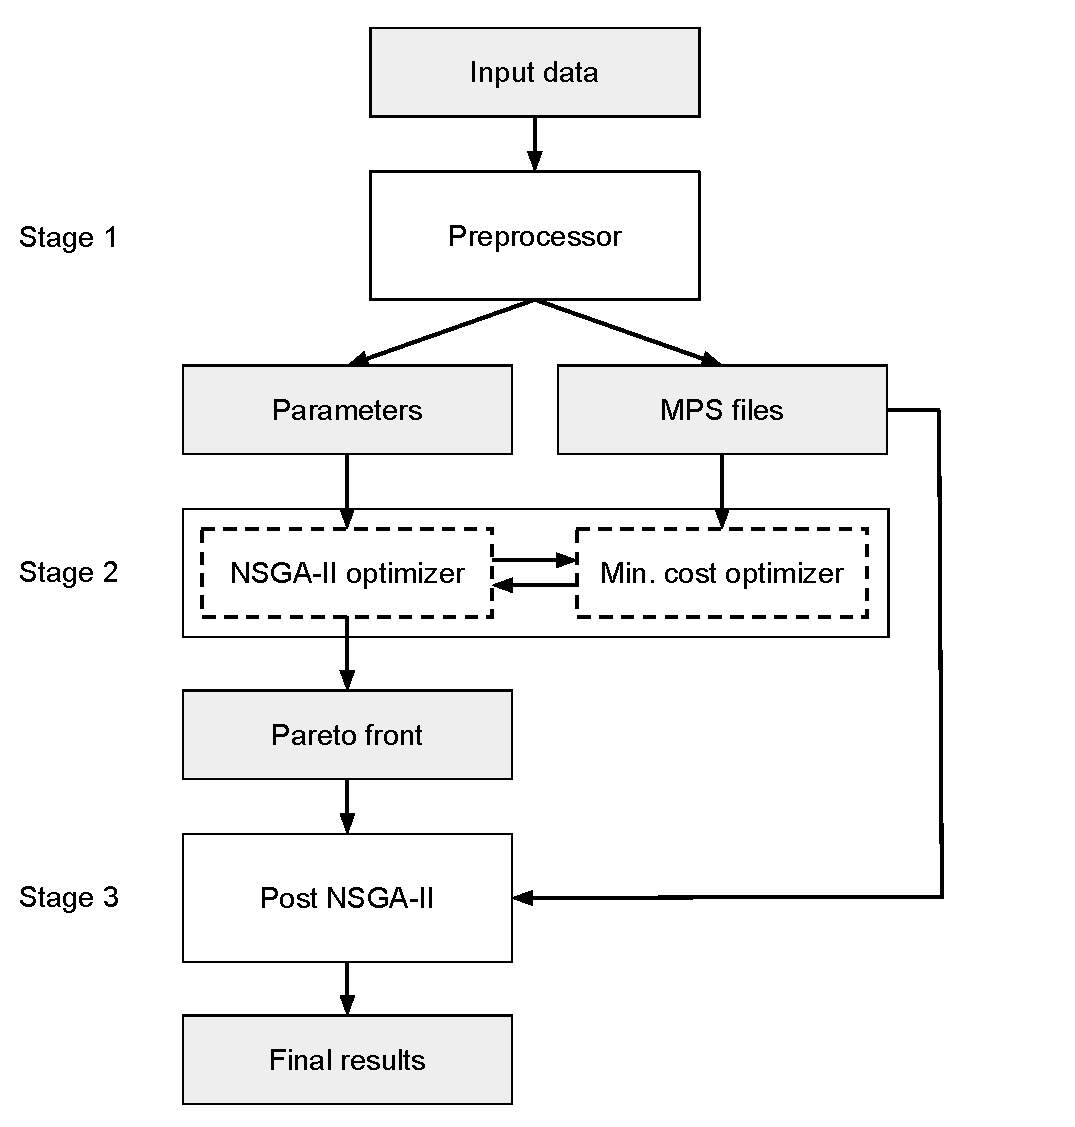
\includegraphics[width=100mm]{figs/software_structure}
  \caption{Software structure in NETPLAN}
  \label{fig:software_implement}
\end{figure}


The rest of the files are considered libraries and contain auxiliary code for assist the programs above:

\begin{itemize}
  \item \verb=read.cpp=: Functions to read files (global parameters, networks, properties, etc.)
  \item \verb=write.cpp=: Writing files (solutions, temporary files, etc.)
  \item \verb=global.cpp=: Common global definitions
  \item \verb=netscore.h=: Common tasks and misc.
  \item \verb=node.cpp=: Declares a special class to store node information, along with functions to read, modify and write node data
  \item \verb=arc.cpp=: Similar but for arcs
  \item \verb=step.cpp=: Functions related with time and time steps
  \item \verb=index.cpp=: Special variables and functions to store order of arcs and nodes (similar to the a vector index, hence the name)
  \item \verb=solver.cpp=: Functions to solve a problem (includes Benders decompositions)
\end{itemize}


\section{Basic commands}

This is a list of the basic commands that are used to compile and execute the different functions in NETPLAN:

\begin{itemize}
  \item \verb=make=: Compiles the source code
  \item \verb=./prep= (stage 1): Runs the preprocessor, taking the information in the \verb=data= folder and creating the optimization model
  \item \verb=./post=: Evaluates the minimum cost problem after it has been created
  \item \verb=./nsga2= (stage 2): Runs the full multiobjective optimization
  \item \verb=./postnsga= (stage 3): Evaluates the Pareto front solutions
  \item \verb=make clean=: Eliminates the compiled programs (useful to clean the folder back to the original state)
  \item \verb=make cleanmps=: Eliminates results and auxiliary files
\end{itemize}


\section{Constructing a model}

This will be a brief description of how to construct a functioning model. There is a small example in the website that might be helpful to visualize how it is done. References to the different formulation parameters are included.

All the data manipulation is done inside the \verb=data= folder. The following subsections will explain the content of the different files, which use the CSV\footnote{Comma separated values} format. It is recommended using plain-text editors (such as Notepad on Windows) to modify \verb=parameters.csv=. Any other file can be edited with Notepad or Excel 2007 or newer.


\subsection{parameters.csv}

This is the most important file where the global parameters of the optimization are defined. It consists of two columns without a header. The first column is used for keywords and the second for values. The following is a list of the keywords, acceptable inputs or ranges and default values. The last few parameters are specific to NSGA-II.

Some values can be defined here and will be used as defaults. The philosophy is to take the most specific first and then try more relaxed definitions.

Parameters are listed as \verb=keyword= [range] \textbf{default}
\begin{itemize}
  \item \verb=StepName= [letters] \textbf{None}: Definition of the key letters that will used to describe time steps. It is required and it must have one or more letters. E.g., ``ym" would indicate that we are using years and months.
  \item \verb=StepLength= [letters and numbers] \textbf{None}: Definition of the maximum length of the time steps (also required). E.g., ``y2m12" indicates that simulation is 2 years long and each year has 12 months.
  \item \verb=StepHours= [number] \textbf{1}: Defines the length in hours the last member in the time step (``m" in the example). If it used once all time steps will be the same. It can be also be used multiple time to define different time lengths, e.g., to describe different segments on the load duration curve.
  \item \verb=DefStep= [letters as in StepName] \textbf{None}: Defines what is the default time step level for arcs and nodes. E.g., ``ym"
  \item \verb=DefDiscount= [0--1] \textbf{0}: Default discount rate ($r$ in the formulation) that will be applied to all nodes and arcs, unless otherwise specified.
  \item \verb=DefInflation= [0-1] \textbf{0}: Similar to discount but this reflects price inflation.
  \item \verb=DefDemandRate= [number] \textbf{0}: Used to define the rate at which demand grows globally. E.g., ``0.02" means that demands grow 2\% annually by default.
  \item \verb=UseDCFlow= [true/false] \textbf{false}: Use DC power flow equations.
  \item \verb=CodeDC= [two letters] \textbf{None}: Define two letter code to identify nodes that use DC power flow. E.g., ``EL".
  \item \verb=UseBenders= [true/false] \textbf{false}: Use Benders decomposition to solve minimum cost problem.
  \item \verb=OutputLevel= [0--2] \textbf{2}: Level of output on screen (0 for most information).
  \item \verb=TransStep= [letters as in StepName] \textbf{None}: Default transportation step. E.g., ``y" means that all transportation is represented on an annual basis.
  \item \verb=TransInfra= [letters] \textbf{---}: The first letter represents a new transportation infrastructure. The rest are the different modes that can use that infrastructure. E.g., ``rt" adds infrastructure railroad and indicated that t (trains) can use railroad. This command should be used as many time as transportation infrastructures considered.
  \item \verb=TransComm= [letters] \textbf{---}: The first letter defines a new commodity. The rest define what modes can transport the current commodity. E.g., ``1t" indicates that commodity 1 (coal type 1) can travel by train. This command should be repeated for each commodity.
  \item \verb=TransCoal= [letters] \textbf{None}: The letters correspond to the commodity codes that represent coal, i.e., the members of $\mathcal{K}_c$. The command is to be used once.
  \item \verb=AddObj= [letters and numbers] \textbf{---}: This command adds a new sustainability objective. E.g.,~``emCO2" for CO$_2$ emissions. It can be repeated.
  \item \verb=AddMetric= [letters and numbers] \textbf{---}: Similar to the above but it creates a metric that is not minimized, just reported.
  \item \verb=NumberEvents= [integer] \textbf{0}: Declares the number of events to be used for resiliency. E.g.,~``2".
  \item \verb=popsize= [multiple of 4] \textbf{20}: Population size for a generation (NSGA-II).
  \item \verb=ngen= [number] \textbf{200}: Number of generations (NSGA-II).
  \item \verb=pcross_real= [0--1] \textbf{0.75}:  Crossover probability for real variables (NSGA-II).
  \item \verb=pmut_real= [0--1] \textbf{0.4}:  Mutation probability for real variables (NSGA-II).
  \item \verb=eta_c= [number] \textbf{7}:  Distribution index for real variable SBX crossover (NSGA-II).
  \item \verb=eta_m= [number] \textbf{20}:  Distribution index for real variable polynomial mutation (NSGA-II).
  \item \verb=pcross_bin= [0--1] \textbf{0.4}:  Crossover probability for binary variables (NSGA-II).
  \item \verb=pmut_bin= [0--1] \textbf{0.5}:  Mutation probability for binary variables (NSGA-II).
  \item \verb=stages= [integer] \textbf{2}:  Number of bits used to represent an investment (NSGA-II).
  \item \verb=pstart= [0--1] \textbf{0.5}:  Probability that each of the bits takes the value of 1 for the first randomly generation (NSGA-II).
\end{itemize}


\subsection{node\_List.csv}

This file defines the set of energy nodes, $\mathcal{N}^E$. Nodes are named the following way: ``CMIAy1m1", where the characters represent:

\begin{itemize}
  \item First character is energy network: coal, electricity, etc.
  \item Second character is node type: Coal steam generator, storage, transmission
  \item Third and fourth are location: Iowa, Northwest Power Pool Area, etc.
  \item The rest refer to time step: month 1 of year 1, year 2, etc.
\end{itemize}

In this file we define the first four characters, i.e. network, type and location (e.g., ``CMIA"). NETPLAN takes care of adding the time information. The first line of the file is reserved for the header. Starting on the second line, each line is occupied by the definition of a node. Of course, each node code needs to be unique. The first lines would go like the following (note that anything after the \% is considered a comment and it's omitted).

\begin{verbatim}
     code
     % Coal production nodes
     CPAL
     CPAZ
     CPAR
     CPCO
     ...
\end{verbatim}


\subsection{arcs\_List.csv}

An arc is simply determined by the origin and destination nodes with a separation character, in the following fashion: ``ETIAy1m1\_ETMNy1m1". In this example we would be representing the electric transmission from Iowa to Minnesota for the first month of the first year.

Similar to the previous file, the first line is reserved for the header. After that, each line defines the four character code for origin and destination node in the first and second columns, respectively. For example:

\begin{verbatim}
     from,to
     % Coal production to transportation node,
     CPAL,2TAL
     CPAZ,4TAZ
     CPAR,3TAR
     ...
\end{verbatim}


\subsection{trans\_List.csv}

This file introduces the transportation variables, $f_{(i,j,k,m)}(t)$: flow of transportation arc from node $i$ to node $j$ for commodity $k$ using transportation mode $m$ during time step $t$) are coded like this: ``ttMONEy1\_1TMONEy1":

\begin{itemize}
  \item In the first half, the first two letters are the same and represent the transportation mode (train in this case)
  \item The next two characters represent the origin (here is Missouri)
  \item Destination code is defined in the next two characters (Nebraska in this case)
  \item The remaining characters before the underscore (\_) represent time step (year 1)
  \item The second half begins with the commodity character (1 represents coal)
  \item The next character is always a ``T" to represent transportation.
  \item The remaining characters are repeated from the first part (origin, destination, time).
\end{itemize}

NETPLAN uses the definition of commodities, infrastructures and modes from the global parameters to simplify the definition of the transportation network. This file starts with a line reserved for the header and then each line is composed by four columns:

\begin{itemize}
  \item Origin two character code
  \item Destination two character code
  \item Distance in miles
  \item Characters to represent fleets allowed on that connection (if left blank, all fleets are used for that link)
\end{itemize}

This is an example:

\begin{verbatim}
     from,to,mileage,fleet
     AL,FL,591.5,
     AL,GA,182,t
     AL,MS,207.5,k
     ...
\end{verbatim}

The transportation network is then coded into arcs and nodes, compatible with the energy network definition. In the example above a node called ``1TMONEy1" would be created. It is this node that should be used to enter the transportation load for commodity ``1" between ``MO" and ``NE".


\subsection{Simplification for data storage}

Before we continue, it is worth describing how data is stored in the rest of the files. This system is aimed at reducing the number of entries so that new cases can be modified quickly.

Let's say for example that we want to establish the efficiency of all transmission lines to 98\%, for all locations and all time steps. In that case we could assign a value of 0.98 for efficiency using the following entry.

\begin{verbatim}
     EL_EL   0.98
\end{verbatim}

Using this simplified method we reduce the number of necessary data entries (and thus the chances of making errors) and it is much easier to modify later. The code I am preparing is capable of extending the simple above to all the arcs were it is required.

Now assume that we want to say that the wind generation units in Texas have a cost of 0.2, for all time steps. The necessary entry would be:
\begin{verbatim}
     EWTX_ETTX   0.2
\end{verbatim}

When dealing with time, I have been using the following scheme:

\begin{verbatim}
             const   y1     y2   ...   y1m1   y1m2   ...   y2m1   ...
     ET_ET   0.98    0.95        ...          0.87   ...          ...
\end{verbatim}

The above is a table of possible values of efficiencies for all electric transmission lines for different times. The way is setup allows minimizing the number of entries with respect to time steps. Note that there are empty cells in the table above. The steps to follow when you read the table are:
\begin{itemize}
  \item Check if there is a value available in the smallest time step.
  \begin{itemize}
    \item If such a value exists, take it. Example: 0.87 for y1m2.
    \item If it doesn't, continue. Example: y1m1
  \end{itemize}
  \item Check the following time step that includes the previous one:
  \begin{itemize}
    \item If there is a value, take it. Example: 0.95 for y1
    \item If there isn't, continue. Example: y2
  \end{itemize}
  \item Continue until reaching the constant value.
\end{itemize}

In the case above, some values would be the following:
\begin{itemize}
  \item y1m1 = 0.95
  \item y1m2 = 0.87
  \item y2m1 = 0.98
\end{itemize}


\subsection{nodes\_[Parameter].csv}

All the remaining files that follow this nomenclature are used to define the rest of parameters in the model for nodes. This list presents these parameters, where the \verb=keyword= is part of the file name (e.g., \verb=nodes\_Demand.csv=):

\begin{itemize}
  \item \verb=Step= [characters in StepName] \textbf{DefStep}: Time step for a particular node
  \item \verb=Demand= [number/X] \textbf{0}: Fixed demand at the node ($d^E_j(t)$ or $d^T_{(i,j,k)}(t)$). If ``X" is used, demand equations \ref{eqn:Edemand} and \ref{eqn:Tdemand} are not enforced.
  \item \verb=DemandPower= [number/X] \textbf{X}:  Definition of Demand in terms of power. If ``X" is used, demand defaults to the previous parameter
  \item \verb=DemandRate= [number] \textbf{DefDemandRate}: This parameter can be used to simulate a fixed annual increase in the demand.
  \item \verb=CostUD= [number/X] \textbf{X}:  If different than ``X", a variable representing unserved demand is introduced and the cost is a penalty for not serving that demand.
  \item \verb=DiscountRate= [number] \textbf{DefDiscountRate}: Discount rate to be applied to \verb=CostUD=.
  \item \verb=InflationRate= [number] \textbf{DefInflationRate}: Inflation rate to be applied to \verb=CostUD=.
  \item \verb=PeakPower= [number/X] \textbf{X}:  If different than ``X", constraints are created so that meeting peak power is enforced.
  \item \verb=PeakPowerRate= [number] \textbf{0}: Annual rate to be applied to peak power.
\end{itemize}


\subsection{arcs\_[Parameter].csv}

Similarly, the remaining parameters for arcs are defined here. This is a list, including the \verb=keyword= that needs to be used in the file name.

\begin{itemize}
  \item \verb=OpCost= [number] \textbf{0}:  Operational cost for an arc.
  \item \verb=InvCost= [number/X] \textbf{X}: If different than ``X", investment is allowed on the arcs, using this investment cost.
  \item \verb=DiscountRate= [number] \textbf{DefDiscountRate}: Discount rate to be applied to operational and investment costs.
  \item \verb=InflationRate= [number] \textbf{DefInflationRate}: Inflation rate to be applied to operational and investment costs.
  \item \verb=Distance= [number/X] \textbf{X}: If different than ``X", it becomes a multiplier of costs. Thus, the input of costs is in per mile terms.
  \item \verb=Eff= [number] \textbf{1}:  Arc efficiency
  \item \verb=OpMin= [number] \textbf{0}: Minimum operational flow.
  \item \verb=OpMax= [number/Inf] \textbf{}: Capacity at the arc due to existing infrastructure at time 0. No capacity is enforced if defined as ``Inf".
  \item \verb=InvMin= [number] \textbf{0}:  Minimum investment on the arc.
  \item \verb=InvMax= [number/Inf] \textbf{Inf}:  Maximum investment on the arc.
  \item \verb=InvStart= [time step] \textbf{First time step}: Defines when the first investment is allowed.
  \item \verb=LifeSpan= [time step/X] \textbf{X}:  If different than ``X" investments have a predetermined life span.
  \item \verb=Suscep= [number/X] \textbf{X}:  If different than ``X", the arc is endowed with susceptance and included in the DC power flow equations.
  \item \verb=CapacityFactor= [number] \textbf{0}:  If bigger than 0, the arc is taken into account to meet peak demand at the destination node.
  \item \verb=OpSUST= [number] \textbf{0}: Coefficient to add the current arc to the calculation of a sustainability objective or metric. Substitute ``SUST" by the appropriate code used in the parameter file.
\end{itemize}



\subsection{arcs\_TransEnergy.csv}

This file defines the fuel consumption of fleet, $\emph{fuelCons}_{(i,j,m)}(t)$, which creates extra demand on the energy side. The first row is reserved as a header. After that, one must write blocks of rows corresponding to the fuel consumption. Thus, a transportation link can create demand in multiple energy nodes.

The first column is matched to the first portion of the transportation arc. The second is used to define the four character code of the energy node to add demand. In the example below, the train (represented by the character \verb=t=) creates a demand of 170.5 MMBtu per million ton-mile transported in nodes ``DT01" and ``DT02", that is diesel nodes at location ``01" and ``02".

\begin{verbatim}
     from,to,const
     tt0102,DT01,170.5 % MMBtu/MMton-mile
     tt0102,DT02,170.5
     kk0102,DT01,1678.5
     kk0102,DT02,1678.5
\end{verbatim}


\subsection{events/CapacityLossN.csv}

The files in the \verb=events= folder are used to define the events to calculate resiliency metrics. Substitute ``N" by the appropriate event number (from 1 up to the maximum defined in the global parameters) in the file name.

Within these files we define the fraction of capacity that is available due to a contingency. If not explicitly defined, NETPLAN will use the default of 1 and assume that the capacity was not lost. For example, the entry below indicates that pulverized coal generators are available at 70\% during the second year.

\begin{verbatim}
     from,to,y2
     EC,,0.7
\end{verbatim}

The software automatically identifies which are the operational years affected for each event in order to perform the minimum number of calculations that are necessary.


\section{Modeling Approach} \label{sec:approach}

The energy system is comprised of (but not limited to) electricity, natural gas, liquid fuels, nuclear, biomass, hydroelectric, wind, solar, and geothermal resources. Modeling of national freight and passenger transportation focuses on state-to-state travel; we consider both infrastructures (rail, highways, locks/dams, roads, ports, airports) and fleets (trains, barges, trucks, personal vehicles, airplanes, etc.), and there may be different kinds of fleets for each mode (e.g., diesel trains and electric trains or conventional and plug-in hybrid electric).

\begin{figure}
\begin{center}
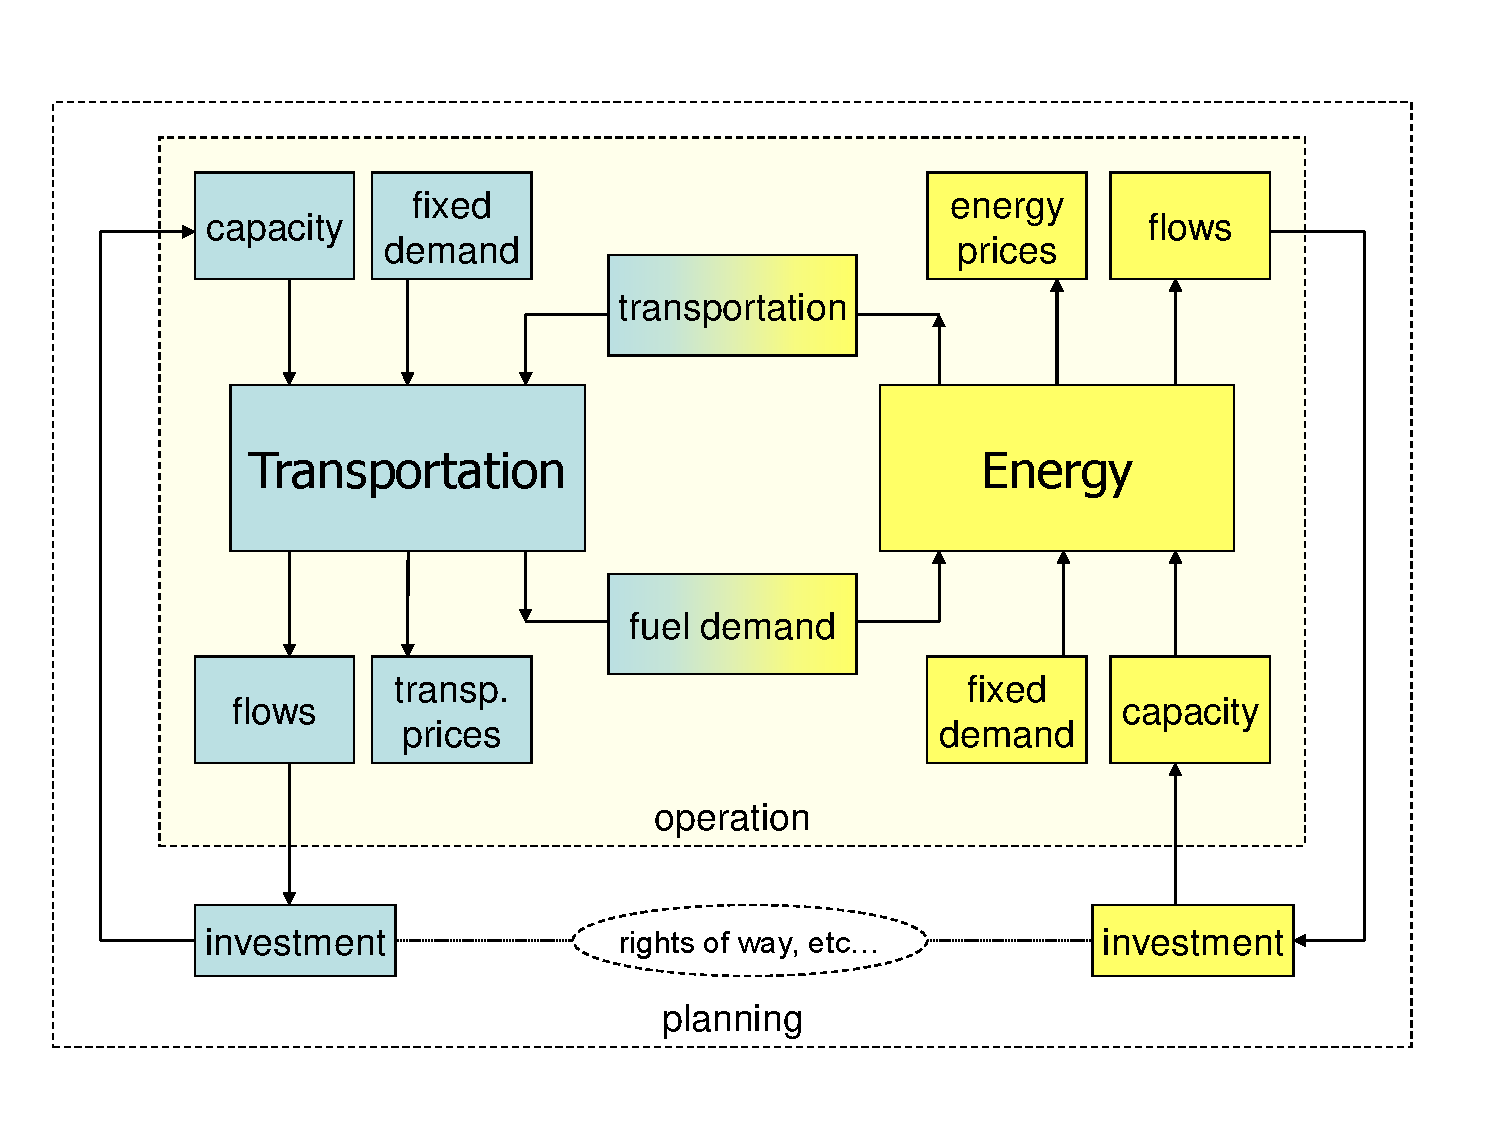
\includegraphics[width = 100mm]{figs/modeling_approach}
\end{center}
\caption{Proposed model that integrates the energy and transportation systems at two levels: operation and planning}
\label{fig:proposedmodel}
\end{figure}

Fig.~\ref{fig:proposedmodel} captures the scope of the modeling effort. The transportation and energy systems interact mainly at two different stages: operation and investment. At the operational level each system needs to satisfy its demand with the existing capacity. However, operation of the two systems, and ultimately investment, are interdependent; while the transportation sector demands energy in the form of fuel, the energy sector requires the movement of raw bulk energy sources (e.g. coal or natural gas for thermal power plants). At the same time, the cost of meeting those reciprocal demands has an impact on final prices for energy and transportation. The ever-growing public need for energy and transportation creates the necessity to invest in new capacity. Given the potential for increased coupling between energy and transportation, it is apparent that better designs of both can be achieved if these designs are performed together.

Our modeling approach consists of two levels. The lower level performs a cost minimization on a 40 year infrastructure investment plan, constrained by lower and upper limits on technology investments, and evaluates resiliency and sustainability metrics. The higher level uses an evolutionary program to perform a multiobjective search for the Pareto optimal front in the space of cost, resiliency, and sustainability metrics, by manipulating the technology investment lower and upper limits. The remainder of this section, together with Section 3, is devoted to describing the lower level. The higher level is described in Section 4.

\subsection{Energy systems modeling}
A generalized network flow transportation model \cite{quelhas1,quelhas2,gil_katrina} is used to model energy systems, where commodity flow is energy, and transportation paths are AC and DC electric transmission, gas pipelines (for natural gas and/or hydrogen), and liquid fuel pipelines (for petroleum-based fuels, biofuels such as ethanol or biodiesel, and anhydrous ammonia). Energy transport by rail, barge, and truck is included in the freight transport model.

Each source node, specified with location, is connected to a fictitious source node that supplies all energy. Arcs emanating from each source are characterized by maximum extraction rate and extraction cost. Petroleum, coal, natural gas, and uranium have finite capacities, while renewables have infinite capacities. All sources have finite maximum extraction rates. Conversion and transportation are endowed with: capacity, efficiency, operational cost, investment cost, lifetime, component sustainability metrics (e.g., CO$_2$), and component resiliency (e.g., reliability).

\subsection{Transportation systems modeling}
The freight transport system is modeled as a multicommodity flow network where the flows are in the units of tons of each major commodity. A commodity is major if its transportation requirements comprise at least 2\% of the nation's total freight ton-miles. Data available to make this determination~\cite{DOT_Forecasts} indicates this criterion includes 23 commodities that comprise 90\% of total ton-miles (e.g., the top eight, comprising 55\%, are in descending order: coal, cereal grains, foodstuffs, gasoline and aviation fuel, chemicals, gravel, wood products, and base metals).

There are two fundamental differences between this formulation and that of the energy formulation. Whereas the energy formulation must restrict energy flows of specific forms to particular networks (for example, natural gas or hydrogen cannot move through electric lines or liquid fuel lines), commodities may be transported over any of the transport modes (rail, barge, truck). Also whereas energy movement requires only infrastructure (electric lines, liquid fuel pipelines, gas pipelines), commodity movement requires infrastructure (rail, locks/dams, roads, ports) and fleet (trains, barges, trucks), and there may be different kinds of fleets for each mode (e.g., diesel trains or electric trains).

To accommodate these differences, the transportation formulation is comprised of two multicommodity flows~\cite{linear_programming}, one embedded inside the other. Commodities flow through the network formed by the different types of fleet available. At the same time, the units in those fleets travel along the network formed by the different infrastructures. An easy way to visualize this is captured in Fig.~\ref{fig:decomposition}, where the flow from node A to node B is divided according to the types of infrastructures first and then into the different types of available fleets.

\begin{figure}[ht]
\begin{center}
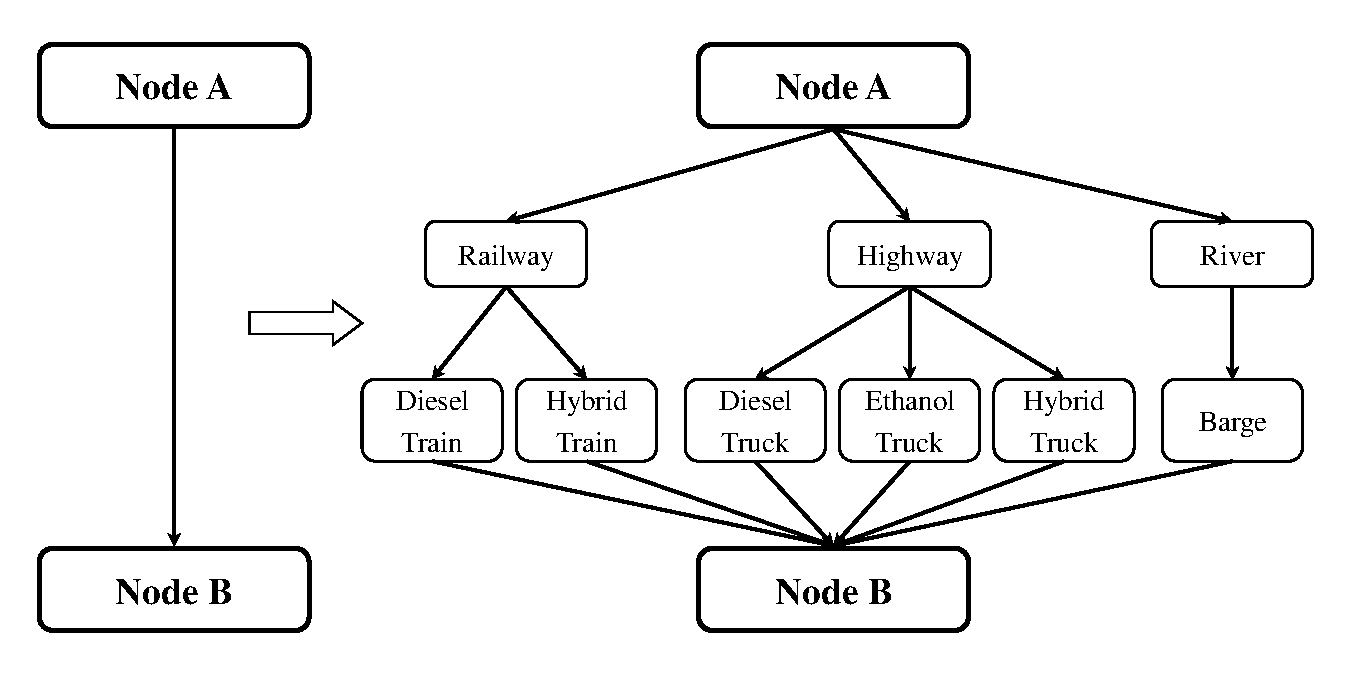
\includegraphics[width=100mm]{figs/transportation}
\end{center}
\caption{Decomposition of transportation arc in two steps: infrastructure and fleet.}
\label{fig:decomposition}
\end{figure}


\section{General cost minimization formulation}
The optimization problem associated with this model can be conceptually described by (\ref{eqn:basic}),

\begin{align}
\begin{split}
& \textbf{min}\quad \emph{CostOp}+\emph{CostInv}\\
& \textbf{subject to:}\\
& \emph{Meet energy demand},\\
& \emph{Meet transportation demand},\\
& \emph{Capacity constraints}\\
& \emph{Power flow constraints on electric transmission}\\
\end{split}\label{eqn:basic}
\end{align}

The objective is to minimize the combined energy and a transportation cost with constraints of meeting demands on energy, and freight transport while following the capacity constraints. The operational characteristics of the model provide additional constraints on the system, such as the inclusion of power flow relations for electric transmission lines (we used the so-called ``DC'' power flow approximation for this purpose).

This section contains a rigorous description of the formulation needed to achieve the characteristics described above. The explanation of the formulation is preceded by an introduction to the nomenclature used.


\subsection{Nomenclature}

\subsubsection{Decision Variables}

\begin{description}
\item $e_{(i,j)}(\textbf{t})$: Operational flow of energy arc from node $i$ to node $j$, for time step \textbf{t} (MWh)
\item $\emph{eInv}_{(i,j)}(\textbf{t})$: Capacity investment on energy arc from node $i$ to node $j$, for time step \textbf{t}. (MW)
\item $f_{(i,j,k,m)}(\textbf{t})$: Operational flow of transportation arc from node $i$ to node $j$ for commodity $k$ using transportation mode $m$ during time step \textbf{t} (ton)
\item $\emph{fleetInv}_{(i,j,m)}(\textbf{t})$: Fleet $m$ capacity investment for transportation arc from node $i$ to node $j$ during time step \textbf{t} (ton/hour)
\item $\emph{infInv}_{(i,j,l)}(\textbf{t})$: Infrastructure $l$ capacity investment for transportation arc from node $i$ to node $j$ for time step \textbf{t} (ton/hour)
\item $\theta_i(\textbf{t})$: Phase angle at node $i$, used to model DC power flow (radians)
\end{description}


\subsection{Sets and networks}

\begin{description}
\item $\mathcal{N}^E$: Set of energy nodes
\item $\mathcal{N}^E_d \subset \mathcal{N}^E$: Subset of energy nodes where demand equations are enforced
\item $\mathcal{N}^E_p \subset \mathcal{N}^E$: Subset of energy nodes where peak demand equations are enforced
\item $\mathcal{A}^E$: Set of energy arcs
\item $\mathcal{A}^E_{DC} \subset \mathcal{A}^E$: Set of AC electric transmission arcs, which satisfy DC power flow equations
\item $\mathcal{N}^T$: Set of transportation nodes
\item $\mathcal{A}^T$: Set of transportation arcs
\item $\mathcal{A}^T_j \subset \mathcal{A}^T$: Subset of transportation arcs that create an energy demand at energy node $j$
\item $\mathcal{K}$: Set of commodities
\item $\mathcal{K}_e \subset \mathcal{K}$: Subset of commodities used by the energy system, e.g. coal
\item $\mathcal{M}$: Set of fleet or transportation modes
\item $\mathcal{M}_l \subset \mathcal{M}$: Subset of fleet that can use transportation infrastructure $l$
\item $\mathcal{M}_j \subset \mathcal{M}$: Subset of fleet that require energy from energy node $j$
\item $n^E_{(i,k)} \in \mathcal{N}^E$: Energy node that corresponds to the geographic location $i$  and commodity $k$ in the transportation system
\end{description}


\subsection{Time and time steps}

\begin{description}
\item $\mathcal{T} = [1, \ldots, T_1] \times [0, \dots, T_2] \times \ldots \times [0, \ldots, T_s]$: Definition of simulation time domain, which is divided in $s$ time steps. Time step $i$ is divided into $T_i$ segments. For instance, simulation time could be divided in ``years'', ``months'' and ``days'' with the appropriate number of divisions within each step
\item $\textbf{t} = [t_1, t_2, \ldots, t_s] \in \mathcal{T}$: Time instance in the simulation domain
\item $\textbf{t}_1$: Value of the top level step for time \textbf{t}, i.e., $t_1$
\item $\mathcal{T}_\textbf{t}$: Time that spans between the beginning of the simulation and time \textbf{t}
\item $\Delta(\textbf{t})$: Length of time step \textbf{t} (h)
\end{description}


\subsection{Energy Parameters}

\begin{description}
\item $\eta_{(i,j)}(\textbf{t})$: Efficiency of arc ($i,j$) during time \textbf{t} (unitless)
\item $\emph{lbe}_{(i,j)}(\textbf{t})$: Lower bound for flow in arc ($i,j$) for time \textbf{t} (MWh)
\item $\emph{ube}_{(i,j)}(\textbf{t})$: Upper bound for flow in arc ($i,j$) during time \textbf{t} due to the initial existing infrastructure (MW)
\item $\emph{lbeInv}_{(i,j)}(\textbf{t})$: Minimum allowed capacity increase in arc ($i,j$) at time \textbf{t} (MW)
\item $\emph{ubeInv}_{(i,j)}(\textbf{t})$: Maximum allowed capacity increase in arc ($i,j$) at time \textbf{t} (MW)
\item $\emph{eLife}_{(i,j)}$: Expected lifetime for investments in arc ($i,j$) at time \textbf{t} (year)
\item $\emph{costOp}_{(i,j)}(\textbf{t})$: Operational cost for flow in arc ($i,j$) during time \textbf{t} (\$/MWh)
\item $\emph{costInv}_{(i,j)}(\textbf{t})$: Investment cost for capacity increase in arc ($i,j$) in network $l$, at time \textbf{t} (\$/MW)
\item $\emph{heatContent}_k(\textbf{t})$: Heat content of commodity $k$, at time \textbf{t} (MWh/ton)
\item $d^E_j(\textbf{t})$: Fixed energy demand at node $j$ during time \textbf{t} (MWh)
\item $\emph{peakD}^E_j(\textbf{t})$: Peak demand at electric node $j$ during time \textbf{t} (MWh)
\item $\emph{cf}_{(i,j)}(\textbf{t})$: Capacity factor of generation between nodes $i$ and $j$ at time \textbf{t} (unitless)
\item $b_{(i,j)}$: Susceptance of transmission line between nodes $i$ and $j$ (p.u.)
\end{description}


\subsection{Transportation Parameters}

\begin{description}
\item $\emph{ubFleet}_{(i,j,m)}(\textbf{t})$: Upper bound for total transportation flow for fleet $m$ in arc ($i,j$) during time \textbf{t} due to the initial existing fleet (ton/h)
\item $\emph{lbFleetInv}_{(i,j,m)}(\textbf{t})$: Minimum allowed capacity increase in arc ($i,j$) for fleet $m$ at time \textbf{t} (ton/h)
\item $\emph{ubFleetInv}_{(i,j,m)}(\textbf{t})$: Maximum allowed capacity increase in arc ($i,j$) for fleet $m$ at time \textbf{t} (ton/h)
\item $\emph{fleetLife}_{(i,j,m)}$: Expected lifetime of fleet $m$ in arc ($i,j$) (years)
\item $\emph{ubInf}_{(i,j,l)}(\textbf{t})$: Upper bound for total transportation flow across infrastructure $l$ in arc ($i,j$) during time \textbf{t} due to the initial existing infrastructure (ton/h)
\item $\emph{lbInfInv}_{(i,j,l)}(\textbf{t})$: Minimum allowed capacity increase in arc ($i,j$) for transportation infrastructure $l$ at time \textbf{t} (ton/h)
\item $\emph{ubInfInv}_{(i,j,l)}(\textbf{t})$: Maximum allowed capacity increase in arc ($i,j$) for transportation infrastructure $l$ at time \textbf{t} (ton/h)
\item $\emph{infLife}_{(i,j,k,m)}$: Expected lifetime for infrastructure investment $l$ in arc ($i,j$) (years)
\item $\emph{costOp}_{(i,j,k,m)}(\textbf{t})$: Operational cost for transportation flow in arc ($i,j$) in fleet $m$, commodity $k$ and time \textbf{t} (\$/ton)
\item $\emph{costFleetInv}_{(i,j,m)}(\textbf{t})$: Investment cost for capacity increase in fleet $m$ for arc ($i,j$) and time \textbf{t} (\$ h/ton)
\item $\emph{costInfInv}_{(i,j,l)}(\textbf{t})$: Investment cost for capacity increase in transportation infrastructure $l$ for arc ($i,j$) and time \textbf{t} (\$ h/ton)
\item $\emph{fuelCons}_{(i,j,m)}(\textbf{t})$: Fuel consumption for transportation mode $m$ for transportation arc ($i,j$) during time step \textbf{t} (MWh/ton)
\item $d^T_{(i,j,k)}(\textbf{t})$: Fixed transportation demand of commodity $k$ for arc ($i,j$) during time \textbf{t} (ton)
\end{description}


\subsection{Auxiliary parameters}

These parameters are calculated as a combination of decision variables and predetermined parameters.

\begin{description}
\item $\emph{CostOp}^E$: Operational cost from the energy system (\$)
\item $\emph{CostInv}^E$: Cost due to the investment upgrades on the energy system (\$)
\item $\emph{CostOp}^T$: Operational cost for transportation system (\$)
\item $\emph{CostFleetInv}^T$: Investment cost on transportation fleet (\$)
\item $\emph{CostInfInv}^T$: Cost on transportation infrastructure (\$)
\item $\emph{eCap}_{(i,j)}(\textbf{t})$: Capacity for energy arc from node $i$ to node $j$, for time step \textbf{t}. (MW)
\item $\emph{fleetCap}_{(i,j,m)}(\textbf{t})$: Fleet $m$ capacity for transportation arc from node $i$ to node $j$ during time step \textbf{t} (ton/h)
\item $\emph{infCap}_{(i,j,l)}(\textbf{t})$: Infrastructure $l$ capacity for transportation arc from node $i$ to node $j$ for time step \textbf{t} (ton/h)
\item $d^{ET}_j(\textbf{t})$: Energy demand at node $j$ during time \textbf{t} due to the transportation of commodities (MWh)
\end{description}


\subsection{Other parameters and functions}

\begin{description}
\item $r$: Discount rate
\item $P_E$: Power base for the electric system
\item I[\emph{test}]: Indicator function that equals 1 if \emph{test} is true and 0 otherwise
\end{description}


\section{General formulation}

The following formulation formally incorporates the modeling capabilities that have been described in previous chapters and allow the joint optimization of the transportation and energy networks.

The objective to be minimized (\ref{eqn:objectives}) is the total cost of operating and investment of the combined system. We can distinguish five components in the objective: operational cost of the energy system (\ref{eqn:Eopcost}), investment cost of the energy system (\ref{eqn:Einvcost}), operational cost of the transportation system (\ref{eqn:Topcost}), and investment cost of the transportation system divided into fleet investment (\ref{eqn:Tfleetinvcost}) and infrastructure investment (\ref{eqn:Tinfinvcost}).

The energy sector is represented by a set of nodes $\mathcal{N}^E$ and arcs $\mathcal{A}^E$. Each node represents an energy subnetwork in a geographic location. For example, for a particular location, there might be three energy nodes; one for electricity, one for gas, and one for petroleum. Energy arcs link these various nodes, both within the same subnetwork (representing transmission lines, natural gas pipelines, or petroleum pipelines) or between different networks, where conversion takes place (e.g., power plants).

{\allowdisplaybreaks
\begin{align}
& \textbf{min}\quad \{ \emph{CostOp}^E+\emph{CostInv}^E + \emph{CostOp}^T + \emph{CostFleetInv}^T + \emph{CostInfInv}^T \} \label{eqn:objectives} \\
& \textbf{subject to:} \nonumber \\
& \text{Meet energy demand at the appropriate nodes} \nonumber \\
& \sum_i{\eta_{(i,j)}(\textbf{t}) e_{(i,j)}(\textbf{t})} - \sum_i{e_{(j,i)}(\textbf{t})} = d^E_j(\textbf{t}) + d^\emph{ET}_j(\textbf{t}) \quad j \in \mathcal{N}^E_d \label{eqn:Edemand} \\
& \text{DC power flow equations} \nonumber \\
& e_{(i,j)}(\textbf{t}) - e_{(j,i)}(\textbf{t}) = b_{(i,j)} \Big( \theta_i(\textbf{t}) - \theta_j(\textbf{t}) \Big) \, P_E \, \Delta(\textbf{t}), \quad (i,j) \in \mathcal{A}^E_{DC} \label{eqn:DCpowerflow} \\
& \text{Generation capacity must cover peak demand at electric nodes} \nonumber \\
& \sum_i{\emph{cf}_{(i,j)}(\textbf{t}) \emph{eCap}_{(i,j)}(\textbf{t})} \ge peakD^E_j(\textbf{t}), \quad j \in \mathcal{N}^E_p \label{eqn:Epeak} \\
& \text{Transportation demand for non-energy commodities} \nonumber \\
& \sum_m{f_{(i,j,k,m)}(\textbf{t})} = d^T_{(i,j,k)}(\textbf{t}), \quad k \in \mathcal{K} \char`\\ \mathcal{K}_e \label{eqn:Tdemand} \\
& \text{Transportation demand for energy commodities} \nonumber \\
& \sum_m{f_{(i,j,k,m)}(\textbf{t})} = \emph{heatContent}^{-1}_k(\textbf{t}) \, e_{(n^E_{(i,k)},n^E_{(j,k)})}(\textbf{t}), \quad k \in \mathcal{K}_e \label{eqn:Tcarrier} \\
& \text{Fleet upper bound for transportation flows} \nonumber \\
& \sum_k{f_{(i,j,k,m)}(\textbf{t})} \le \emph{fleetCap}_{(i,j,m)}(\textbf{t}) \, \Delta(\textbf{t}) \label{eqn:Tfleet} \\
& \text{Infrastructure upper bound for transportation flows} \nonumber \\
& \sum_k{ \sum_{m \in \mathcal{M}_l }{ f_{(i,j,k,m)}(\textbf{t}) } } \le \emph{infCap}_{(i,j,l)}(\textbf{t}) \, \Delta(\textbf{t}) \label{eqn:Tinf} \\
& \textbf{Decision variables:} \nonumber \\
& \text{Energy flows:} \qquad 0 \le \emph{lbe}_{(i,j)}(\textbf{t}) \le e_{(i,j)}(\textbf{t}) \le \emph{eCap}_{(i,j)}(\textbf{t}) \, \Delta(\textbf{t}) \label{eqn:Eflow} \\
& \text{Energy capacity inv.:} \qquad \emph{lbeInv}_{(i,j)}(\textbf{t}) \le \emph{eInv}_{(i,j)}(\textbf{t}) \le \emph{ubeInv}_{(i,j)}(\textbf{t}) \label{eqn:Einvvar} \\
& \text{Transportation flows:} \qquad f_{(i,j,k,m)}(\textbf{t}) \ge 0 \label{eqn:Tflow} \\
& \text{Fleet inv.:} \qquad \emph{lbFleetInv}_{(i,j,m)}(\textbf{t}) \le \emph{fleetInv}_{(i,j,m)}(\textbf{t}) \le \emph{ubFleetInv}_{(i,j,m)}(\textbf{t}) \label{eqn:Tfleetvar} \\
& \text{Infrastucture inv.:} \qquad \emph{lbInfInv}_{(i,j,l)}(\textbf{t}) \le \emph{infInv}_{(i,j,l)}(\textbf{t}) \le \emph{ubInfInv}_{(i,j,l)}(\textbf{t}) \label{eqn:Tinfvar} \\
& \text{Phase angles:} \qquad -\pi \le \theta_i(\textbf{t}) \le \pi \label{eqn:angles} \\
& \textbf{where:} \nonumber \\
& \emph{CostOp}^E = \sum_\textbf{t}{\sum_{(i,j)}{(1+r)^{-\textbf{t}_1} \emph{costOp}^E_{(i,j)}(\textbf{t}) \, e_{(i,j)}(\textbf{t})}} \label{eqn:Eopcost} \\
& \emph{CostInv}^E = \sum_\textbf{t}{\sum_{(i,j)}{(1+r)^{-\textbf{t}_1} \emph{costInv}^E_{(i,j)}(\textbf{t}) \, \emph{eInv}_{(i,j)}(\textbf{t})}}  \label{eqn:Einvcost} \\
& \emph{CostOp}^T = \sum_\textbf{t}{\sum_{(i,j,k,m)}{(1+r)^{-\textbf{t}_1} \emph{costOp}^T_{(i,j,k,m)}(\textbf{t}) \, f_{(i,j,k,m)}(\textbf{t})}} \label{eqn:Topcost} \\
& \emph{CostFleetInv}^T = \sum_\textbf{t}{ \sum_{(i,j,m)}{ (1+r)^{-\textbf{t}_1} \emph{costFleetInv}_{(i,j,m)}(\textbf{t}) \, \emph{fleetInv}_{(i,j,m)}(\textbf{t}) } } \label{eqn:Tfleetinvcost} \\
& \emph{CostInfInv}^T = \sum_\textbf{t}{ \sum_{(i,j,l)}{ (1+r)^{-\textbf{t}_1} \emph{costInfInv}_{(i,j,l)}(\textbf{t}) \, \emph{infInv}_{(i,j,l)}(\textbf{t}) } }  \label{eqn:Tinfinvcost} \\
& \emph{eCap}_{(i,j)}(\textbf{t}) = \emph{ube}_{(i,j)}(\textbf{t}) + \sum_{\boldsymbol\tau \in \mathcal{T}_\textbf{t}}{\emph{eInv}_{(i,j)}(\boldsymbol\tau)} \, \textup{I}[\textbf{t}_1 - \boldsymbol\tau_1 \le \emph{eLife}_{(i,j)} ] \label{eqn:Ecap} \\
& \emph{fleetCap}_{(i,j,m)}(\textbf{t}) = \emph{ubFleet}_{(i,j,m)}(\textbf{t}) + \sum_{\boldsymbol\tau \in \mathcal{T}_\textbf{t}}{\emph{fleetInv}_{(i,j,m)}(\boldsymbol\tau)} \, \textup{I}[\textbf{t}_1 - \boldsymbol\tau_1 \le \emph{fleetLife}_{(i,j,m)} ] \label{eqn:Tfleetcap} \\
& \emph{infCap}_{(i,j,l)}(\textbf{t}) = \emph{ubInf}_{(i,j,l)}(\textbf{t}) + \sum_{\boldsymbol\tau \in \mathcal{T}_\textbf{t}}{\emph{infInv}_{(i,j,l)}(\boldsymbol\tau)} \, \textup{I}[\textbf{t}_1 - \boldsymbol\tau_1 \le \emph{infLife}_{(i,j,k,m)}] \label{eqn:Tinfcap} \\
& d^\emph{ET}_j(\textbf{t}) = \sum_{(a,b) \in \mathcal{A}^T_j}{ \sum_{m \in \mathcal{M}_j}{ \emph{fuelCons}_{(a,b,m)}(\textbf{t}) \sum_k{ f_{(a,b,k,m)}(\textbf{t}) } } } \label{eqn:fuel}
\end{align}
}


The flows across these arcs,  $e_{(i,j)}$, are part of the decision variables of the problem. These flows must be such that they satisfy the demand for energy (\ref{eqn:Edemand}), part of which is due to the fuel required to perform the movement of commodities in the transportation system (\ref{eqn:fuel}). Energy flows are also required to meet lower and upper bound constraints (\ref{eqn:Eflow}). Upper bounds are determined by the capacity of the existing energy infrastructure, $\emph{eCap}_{(i,j)}(\textbf{t})$, and are a combination~(\ref{eqn:Ecap}) of the initial capacity, $\emph{ube}_{(i,j)}(\textbf{t})$, and investment on upgrades, $\emph{eInv}_{(i,j)}(\textbf{t})$. The former are given parameters while the latter are also decision variables with their corresponding lower and upper bounds (\ref{eqn:Einvvar}). Energy flows must also satisfy other constraints, such as DC power flow equations for electric transmission (\ref{eqn:DCpowerflow}). Equation (\ref{eqn:Epeak}) ensures that generation for each electric region is able to cover the peak demand.

The transportation system is also formed by a set of nodes $\mathcal{N}^T$ and a set of arcs $\mathcal{A}^T$, although the nomenclature is slightly different. Here each node represents a unique geographic location, while the transportation flows (\ref{eqn:Tflow}) are referred to as $f_{(i,j,k,m)}$, where ($i,j$) represents the origin and destination nodes, $k$ the commodity that is being transported and $m$ the mode of transportation used.

These flows must satisfy the transportation demand, which is predetermined (\ref{eqn:Tdemand}) for all commodities except for those that are energy related (e.g., coal, uranium). In that case transportation demands depend on the use of that commodity in the energy system (\ref{eqn:Tcarrier}). Transportation flows are constrained (\ref{eqn:Tfleet},~\ref{eqn:Tinf}) by the capacity (\ref{eqn:Tfleetcap}) of the available fleet, $\emph{fleetCap}_{(i,j,m)}(\textbf{t})$, and the capacity (\ref{eqn:Tinfcap}) transportation infrastructure $\emph{infCap}_{(i,j,l)}(\textbf{t})$. Both can be increased by the their respective investments,  $\emph{fleetInv}_{(i,j,m)}(\textbf{t})$ and $\emph{infInv}_{(i,j,m)}(\textbf{t})$, which have upper and lower bound constraints (\ref{eqn:Tfleetvar},~\ref{eqn:Tinfvar}).


\subsection{Compact notation}

A more compact version of the previous formulation can be produced using vectorial and matrix notation. First of all, the vector $\textbf{capInv}$ includes all capacity investment variables, while the operational variables are grouped in vectors called $\textbf{flows}_t$. The subscript $t$ in this section represents the top level time step which a variable belongs, i.e., $\textbf{t}_1$ following the notation from the previous section.

When using this notation we can reduce the model to the expressions~(\ref{eqn:matrixform}).

\begin{align}
\begin{split}
& \textbf{min}\quad \begin{bmatrix}
 \textbf{CostInv}^\top & \textbf{CostOp}^\top_1 & \textbf{CostOp}^\top_2 & \ldots \end{bmatrix}
 \begin{bmatrix} \textbf{capInv} \\ \textbf{flows}_1 \\ \textbf{flows}_2 \\ \vdots \end{bmatrix} \\
& \textbf{subject to:} \\
& \qquad \begin{bmatrix}
 -\textbf{I} & \textbf{0} & \textbf{0} & \ldots \\
 \textbf{I} & \textbf{0} & \textbf{0} & \ldots \\
 \textbf{0} & \textbf{A}_1 & \textbf{0} & \ldots \\
 \textbf{0} & -\textbf{I} & \textbf{0} & \ldots \\
 \textbf{L}_1 & \textbf{I} & \textbf{0} & \ldots \\
 \textbf{0} & \textbf{0} & \textbf{A}_2 & \ldots \\
 \textbf{0} & \textbf{0} & -\textbf{I} & \ldots \\
 \textbf{L}_2 & \textbf{0} & \textbf{I} & \ldots \\
 \vdots & \vdots & \vdots & \ddots \end{bmatrix}
 \begin{bmatrix} \textbf{capInv} \\ \textbf{flows}_1 \\ \textbf{flows}_2 \\ \vdots \end{bmatrix}
 \le
 \begin{bmatrix} -\textbf{lbInv} \\ \textbf{ubInv} \\ \textbf{d}_1 \\ -\textbf{lb}_1 \\ \textbf{ub}_1 \\ \textbf{d}_2 \\ -\textbf{lb}_2 \\ \textbf{ub}_2 \\ \vdots \end{bmatrix}
\end{split} \label{eqn:matrixform}
\end{align}

The objective value is (\ref{eqn:objectives}), which is developed in expressions (\ref{eqn:Eopcost}-\ref{eqn:Tinfinvcost}). The first two rows in the constraints are directly related to the minimum and maximum investment allowed (\ref{eqn:Einvvar}, \ref{eqn:Tfleetvar}, \ref{eqn:Tinfvar}).

Following that there are three rows that are repeated for each year. The first two correspond to operational constraints, such as demand balances (\ref{eqn:Edemand}, \ref{eqn:Tdemand}, \ref{eqn:Tcarrier}) or DC power flow constraints (\ref{eqn:DCpowerflow}). Such expressions are summarized in the matrix $\textbf{A}_t$ and the vector $\textbf{d}_t$. The next two lines correspond to the minimum and maximum operational flows from (\ref{eqn:Tfleet}--\ref{eqn:Eflow}, \ref{eqn:Ecap}--\ref{eqn:Tinfcap}). The matrix $\textbf{L}_t$ accounts for the fact that only investments done prior to the operational year can account for available capacity.


\subsection{Multiobjective solver} \label{sec:multiobjective}

NETPLAN, an energy and transportation investment multiobjective evolutionary algorithm is proposed as an approach to efficiently solve the problem described above and produce an approximation to the Pareto front. It has been conceived in a modular fashion, to allow the parallel development of each one of its components. At the highest level two levels can be distinguished, as depicted in Fig.~\ref{fig:multiobjective}.

\begin{figure}
\begin{center}
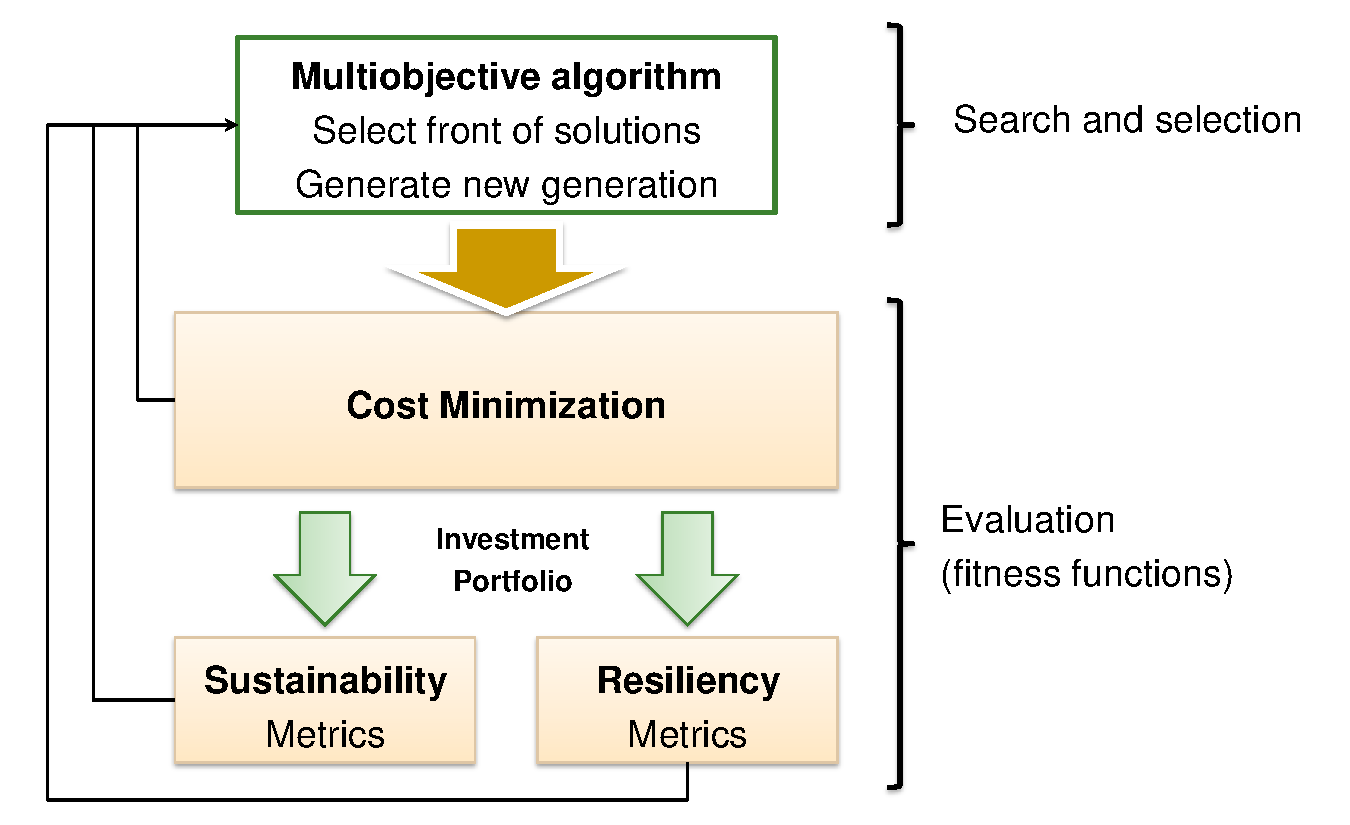
\includegraphics[width=100mm]{figs/multiobjective}
\end{center}
\caption{NETPLAN multiobjective approach}
\label{fig:multiobjective}
\end{figure}

The high-level optimization is directed by the NSGA-II algorithm~\cite{deb}. Each individual within a given population is characterized by a minimum level of investment that is to be enforced. Thus, a vector of minimum values for \emph{capInv} is created for each cost minimization evaluation.

This vector is then passed on to the low-level optimization to be evaluated. This section captures the modeling of the energy and transportation systems, as explained above. First of all, the minimum objective cost problem is solved with the minimum enforced investment constraints incorporated. This process produces the investment portfolio for the individual solutions as well as the flows representing how the system is operated. Other economic factors, such as energy and transportation prices or economic opportunities, can also be extracted.

Once the portfolio is determined, metrics for sustainability and resiliency are calculated. At this stage, those metrics are simple functions based on investments and flows but more complex scenario-based calculations could be implemented using this modular approach.

The objective values are then recovered by the high-level optimization in order to produce the next generation in search for the Pareto front. This loop could also be used to guide the multiobjective optimizer towards a richer variety of solutions. For example, from the dual cost minimization problems one could identify more economic alternatives or, from the evaluation of resiliency, one could identify the weakest links in the system and reinforce them in future solutions. However, including these features would require major modifications in the multiobjective optimizer.

At this point, the use of minimum investment vectors facilitates shifting from the minimum cost solutions to others with better performance in terms of sustainability or resiliency. This approach is very simple to implement but, if needed, could be complemented with other methods such as subsidies for clean alternatives, taxes for polluting technologies (e.g., carbon tax) or preventing certain technologies to be used in favor of others.

\begin{thebibliography}{9}

\bibitem{quelhas1} A.~Quelhas, E.~Gil, J.~McCalley, and S.~Ryan, ``A multiperiod generalized network 
ow model of the U.S.~integrated energy system: Part I - Model description,'' \emph{IEEE Trans.~Power Syst.}, vol. 22, no.~3, pp.~829--836, May 2007.

\bibitem{quelhas2} A.~Quelhas and J.~McCalley, ``A multiperiod generalized network 
ow model of the U.S.~integrated energy system: Part II - Simulation results,'' \emph{IEEE Trans.~Power Syst.}, vol. 22, no.~3, pp.~837--844, May 2007.

\bibitem{gil_katrina} E.~Gil and J.~McCalley, ``A U.S.~energy system model for disruption analysis: Evaluating the effects of
2005 hurricanes,''  \emph{IEEE Trans.~Power Syst.}, vol. PP, no.~99, Jan.~2011.

\bibitem{DOT_Forecasts} U.S.~Department of Transportation, Research and Innovative Technology Administration, Bureau
of Transportation Statistics. (1997) ``Commodity flow survey United States.'' [Online]. Available: \url{http://www.bts.gov/publications/commodity_flow_survey/}

\bibitem{linear_programming} M.~Bazaraa, J.~Jarvis, and H.~Sherali, \emph{Linear Programming and Network Flows}, 2nd ed. New York: Willey, 1990, ch.~12, pp.~587--597.

\bibitem{deb} K.~Deb, A.~Pratap, S.~Agarwal, and T.~Meyarivan, ``A fast and elitist multiobjective genetic algorithm: NSGA-II,'' \emph{IEEE Trans.~Evol.~Comput.}, vol.~6, no.~2, pp.~182--197, 2002.

\end{thebibliography}

\end{document} 